\documentclass[answers]{exam}

%% Language and font encodings
\usepackage[english]{babel}
\usepackage[utf8x]{inputenc}
\usepackage[T1]{fontenc}
% \usepackage{enumitem}
%% Sets page size and margins
\usepackage[a4paper,margin=2cm]{geometry}

%% Useful packages
\usepackage{amsmath}
\usepackage{amssymb}
\usepackage{graphicx}
\usepackage{paralist}
\usepackage{framed}
\usepackage{tikz}
\usepackage{float}
\usepackage{listings}
\usepackage{xcolor}
\tikzset{
  % define the bar graph element
  bar/.pic={
    \fill (-.1,0) rectangle (.1,#1) (0,#1) node[above,scale=1/2]{$#1$};
  }
}
\definecolor{codegreen}{rgb}{0,0.6,0}
\definecolor{codegray}{rgb}{0.5,0.5,0.5}
\definecolor{codepurple}{rgb}{0.58,0,0.82}
\definecolor{backcolour}{rgb}{0.95,0.95,0.92}
% Colored Python listing from https://www.overleaf.com/learn/latex/Code_listing
\definecolor{codegreen}{rgb}{0,0.6,0}
\definecolor{codegray}{rgb}{0.5,0.5,0.5}
\definecolor{codepurple}{rgb}{0.58,0,0.82}
\definecolor{backcolour}{rgb}{0.95,0.95,0.92}
 
\lstdefinestyle{mystyle}{
    backgroundcolor=\color{backcolour},   
    commentstyle=\color{codegreen},
    keywordstyle=\color{magenta},
    numberstyle=\tiny\color{codegray},
    stringstyle=\color{codepurple},
    basicstyle=\ttfamily\footnotesize,
    breakatwhitespace=false,         
    breaklines=true,                 
    captionpos=b,                    
    keepspaces=true,                 
    numbers=left,                    
    numbersep=5pt,                  
    showspaces=false,                
    showstringspaces=false,
    showtabs=false,                  
    tabsize=2
}
\lstset{style=mystyle}

\usetikzlibrary{matrix}

\setlength\FrameSep{4pt}
\title{Probability \& Statistics\\ Project}
\author{Hana Ali Rashid, hr05940\\ Tasmiya Malik, tm06183\\ Ifrah Ilyas, Student ID}
\date{\today{}}
\begin{document}
\maketitle

% \noindent \hrulefill \\
% \textbf{Instructions:}
% \begin{itemize}
%     \item \textbf{Pairs can not be cross-section.}
% \end{itemize}

% \noindent \hrulefill

\section*{Q1: Random Walk}
\subsection*{1.1}
Function implementation in Python:
\lstinputlisting[firstline=5,lastline=13,language=python]{q1.py}
Calling the function for several iterations to get multiple expected values:
\lstinputlisting[firstline=16,lastline=33,language=python]{q1.py}
\pagebreak
Histograms produced by the above code for various combinations of $n$ and $p$:\\
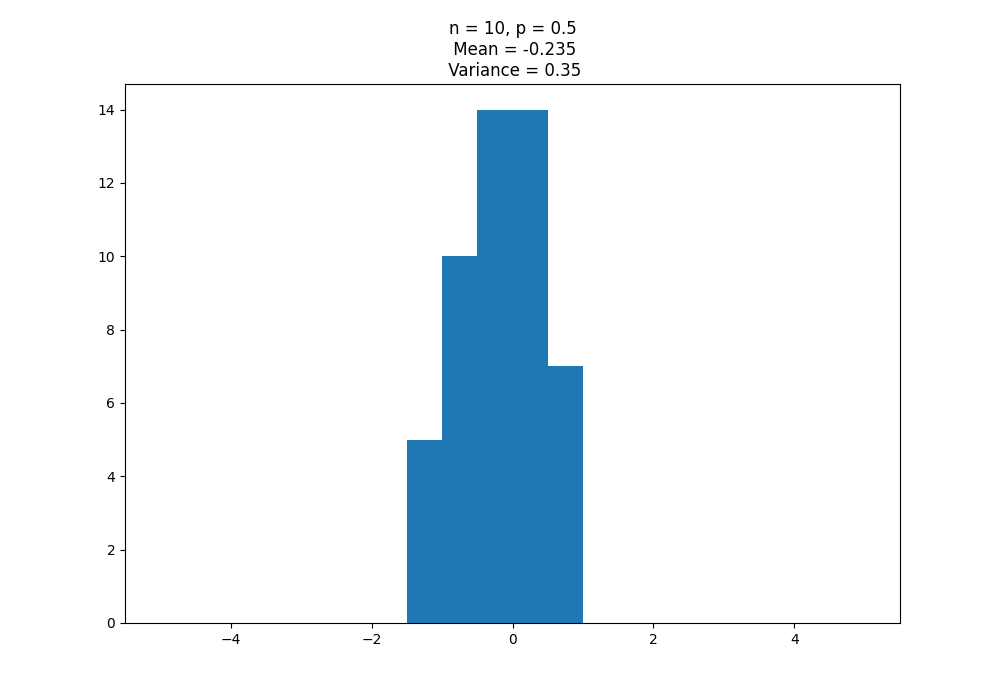
\includegraphics[scale = 0.5]{Q1_histograms/q1_n = 10_ p = 0.5.png}\\
The above histogram appears to follow a normal distribution with a mean of $3.267$ and variance of $0.233$.\\
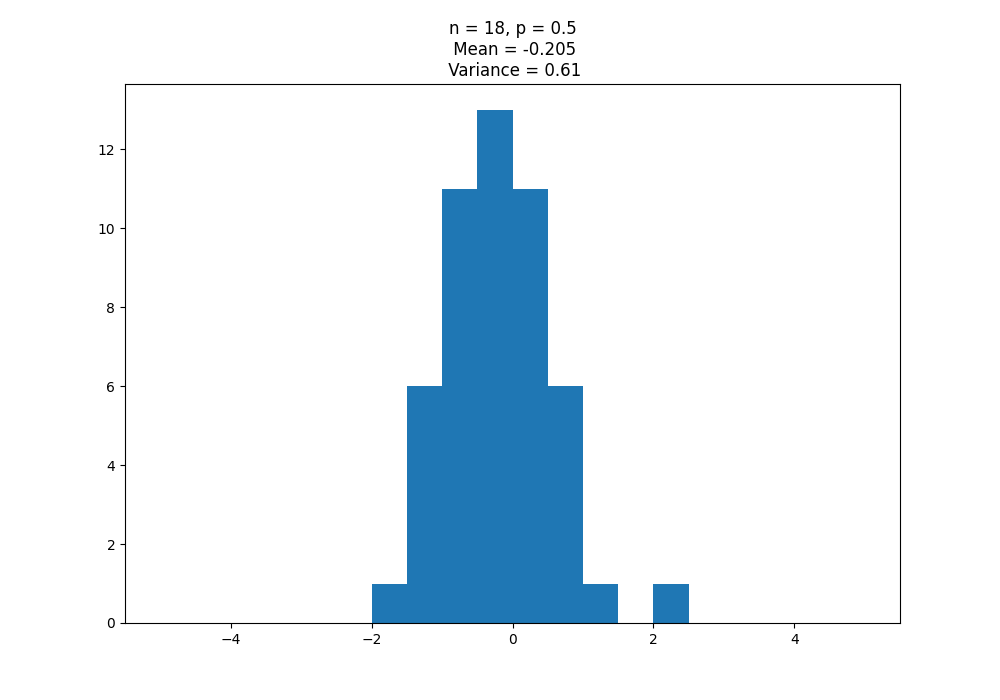
\includegraphics[scale = 0.5]{Q1_histograms/q1_n = 18_ p = 0.5.png}\\
The above histogram appears to follow a normal distribution with a mean of $3.267$ and variance of $0.233$.\\
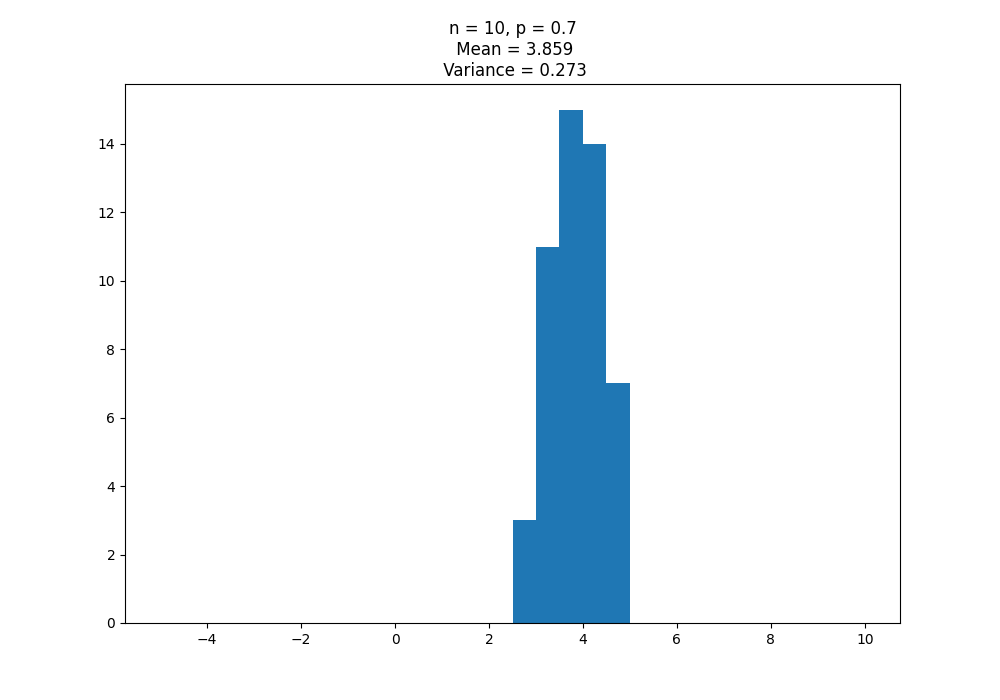
\includegraphics[scale = 0.5]{Q1_histograms/q1_n = 10_ p = 0.7.png}\\
The above histogram appears to follow a normal distribution with a mean of $3.267$ and variance of $0.233$.\\
\pagebreak
%--------------------------------  1.2  ------------------------------------
\subsection*{1.2}
Function implementation in Python:
\lstinputlisting[firstline=36,lastline=44,language=python]{q1.py}
Calling the function for several iterations to get multiple expected values:
\lstinputlisting[firstline=46,lastline=63,language=python]{q1.py}
\pagebreak
Histograms produced by the above code for various combinations of $n$ and $p$:\\
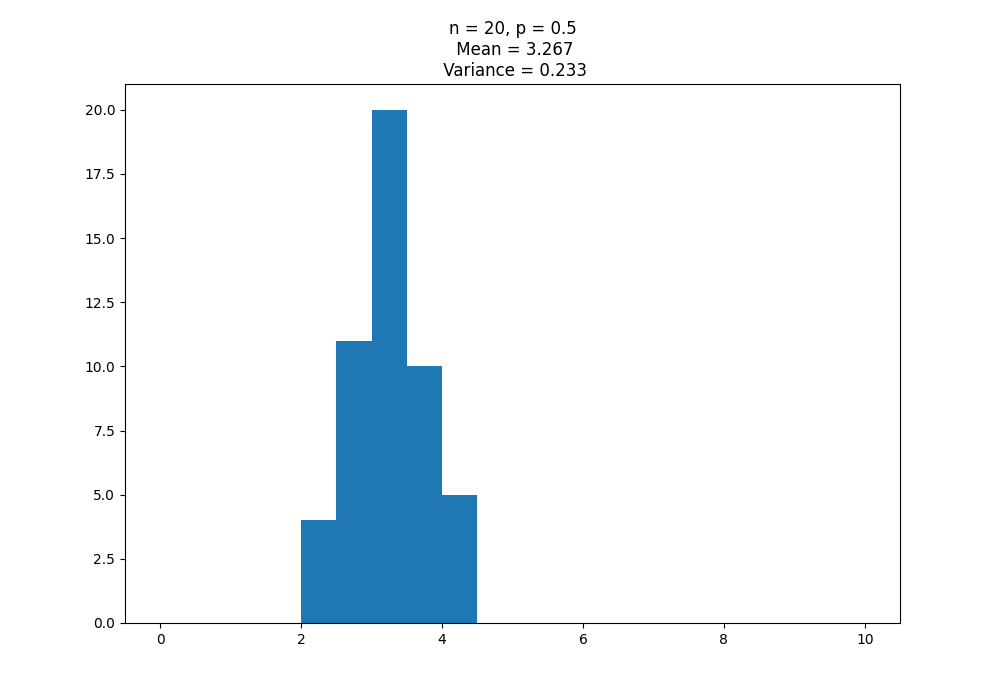
\includegraphics[scale = 0.5]{Q1_histograms/Q1.2 _n = 20_p = 0.5.png}\\
The above histogram appears to follow a normal distribution with a mean of $3.267$ and variance of $0.233$.\\
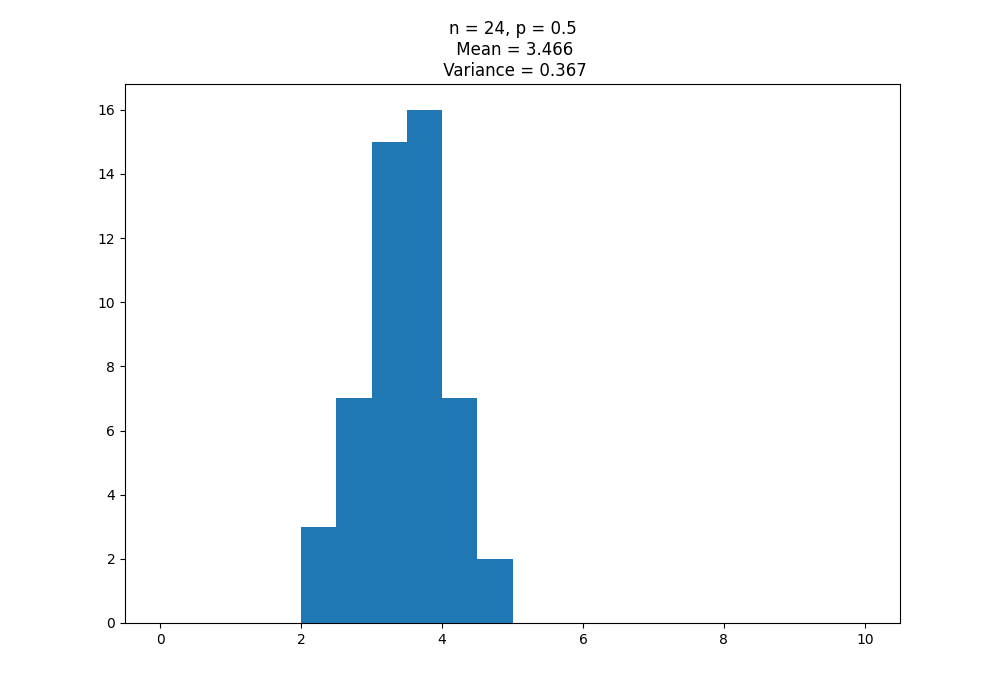
\includegraphics[scale = 0.5]{Q1_histograms/Q1.2 _n = 24_p = 0.5.png}\\
The above histogram shows that...\\
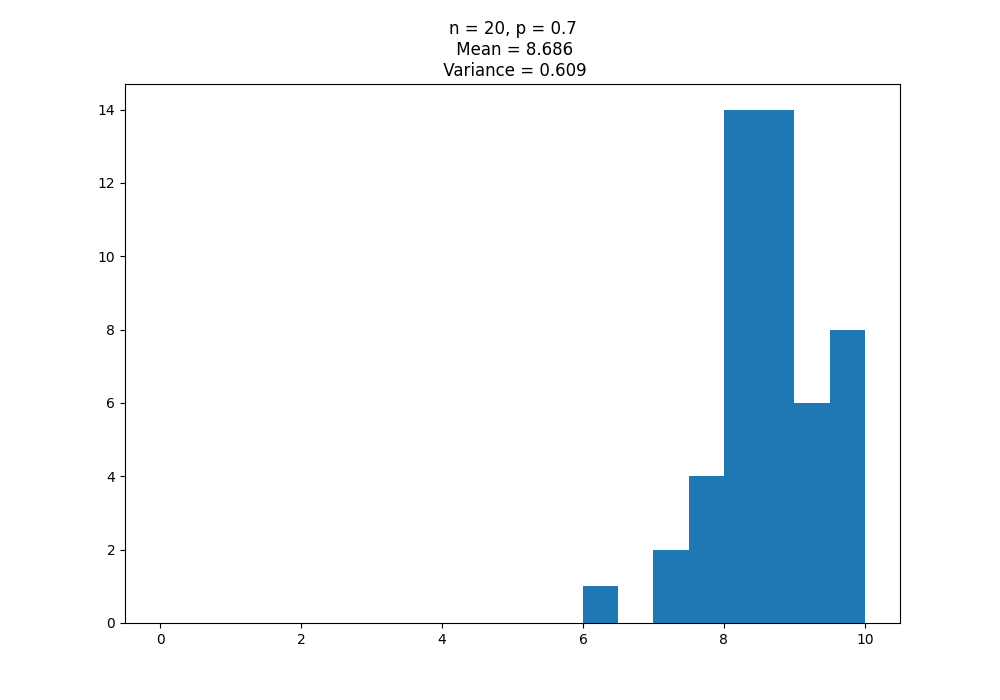
\includegraphics[scale = 0.5]{Q1_histograms/Q1.2 _n = 20_p = 0.7.png}\\
The above histogram shows that...\\
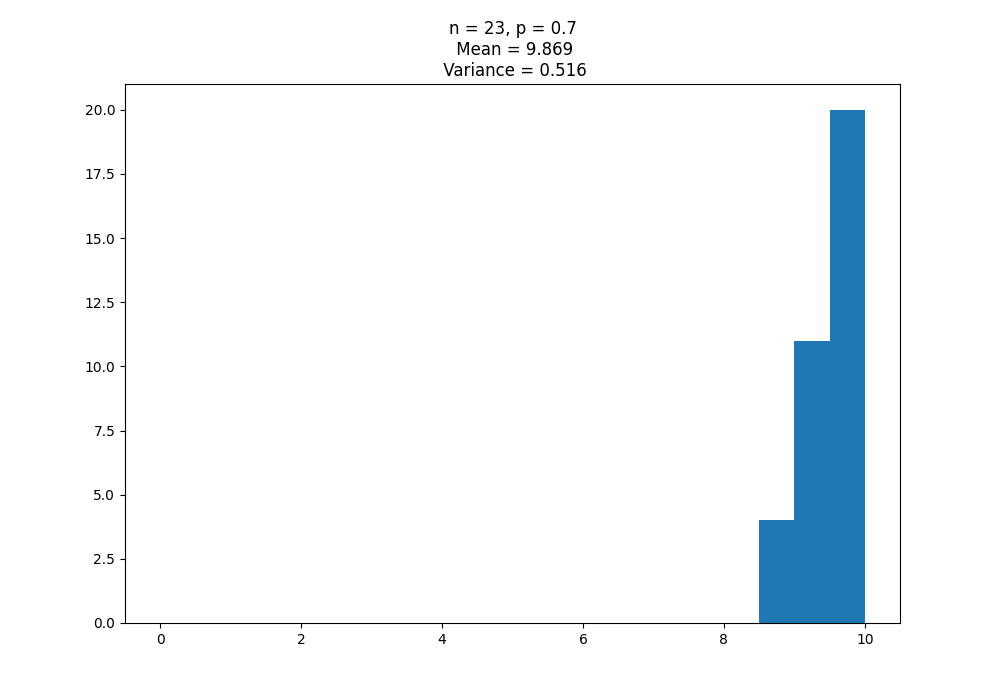
\includegraphics[scale = 0.5]{Q1_histograms/Q1.2 _n = 23_p = 0.7.png}

\pagebreak
%--------------------------------  1.3  ------------------------------------
\subsection*{1.3}
Function implementation in Python:
\lstinputlisting[firstline=65,lastline=79,language=python]{q1.py}
Calling the function for several iterations to get multiple expected values:
\lstinputlisting[firstline=81,lastline=104,language=python]{q1.py}

%--------------------------------  2.*  ------------------------------------



%--------------------------------  3.*  ------------------------------------
\section*{Q3. Picking a Random Point Correctly}

\subsection*{3.1}

\begin{framed}
  For part $3.1$, we followed the method specified in the question. The program takes radius as an input from the user, and passes it to \emph{gen\_points(R)} to display the graph.
  \begin{itemize}
    \item \emph{polar\_to\_cart(r,t)}: This function takes the polar cordinates $(r \text{and} \theta)$ and converts them to their cartesian equivalent. It is called from \emph{polar\_point(R)}, to return the cartesian cordinates.
    \item \emph{polar\_point(R)}: The function is responsible for generating a random point in polar cordinates, and returns the converted cartesian cordinates.
    \item \emph{gen\_points(R)}: This is the main function which runs 1000 iterations, and calls \emph{random\_point(R)}, stores the result in the separate lists for $X$ and $Y$ cordinates. Then the lists are passed to the plot functions, to graph the points.

  \end{itemize}
\end{framed}

\lstinputlisting[firstline=1,lastline=48,language=python]{Prob-Project/Q3/Q3(1).py}

\begin{figure}[h]
  \caption{radius = 100, variance of x = 1626.2176657086331}
  \centering
  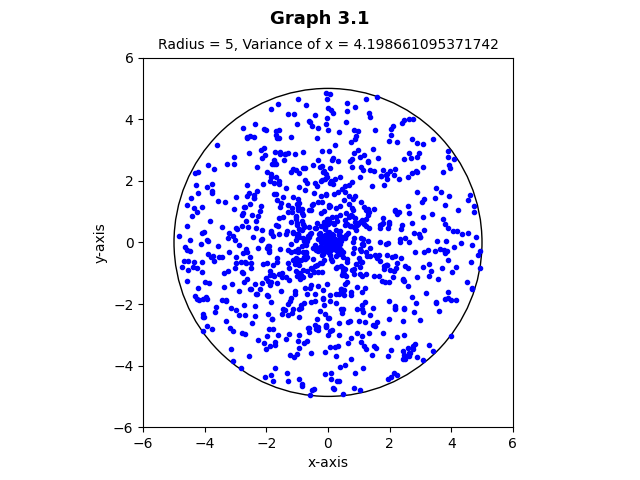
\includegraphics[scale=0.7]{Prob-Project/Q3/Q3(1).png}
\end{figure}

%--------------------------------  3.2  ------------------------------------
\subsection*{3.2}
\begin{framed}
  \indent In part $3.2$, we calculated the cartesian cordinates directly from the specified radius R. If the random point lied farther from the distance from the origin, it will be discarded and the program will find a new point.
  \begin{itemize}
    \item \emph{random\_point(R)}: This function finds random points for $x$ and $y$ cordinates between the range $-R$ and $R$. It returns the tuple with cartesian cordinates.
    \item \emph{dist\_from\_origin(x,y)}: The function find and return the distance of the point from the origin.
    \item \emph{gen\_points(R)}: The main function iterates 1000 times and calls \emph{random\_point(R)}. Then it checks the condition that if the distance of the point $(x,y)$ is within the radius $R$, it would append the points to their respective lists, else the counter will be decremented by 1 and the point will not be added to the list. Then the lists $X$ and $Y$ are passed to the plot functions for display.
  \end{itemize}
\end{framed}
\lstinputlisting[firstline=1,lastline=46,language=python]{Prob-Project/Q3/Q3(2).py}
\begin{figure}[h]
  \caption{radius = 100, variance of x = 2533.130556271337}
  \centering
  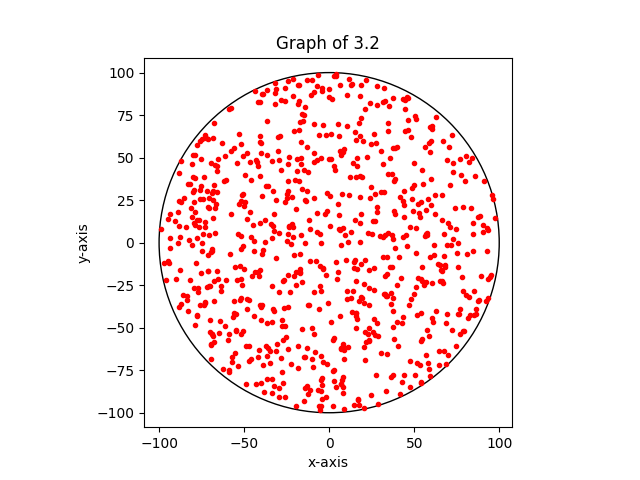
\includegraphics[scale=0.7]{Prob-Project/Q3/Q3(2).png}
\end{figure}


%--------------------------------  3.3  ------------------------------------
\subsection*{3.3}
\begin{framed}
  \indent In part $3.3$, we had to modify the function for polar cordinates, such that the graph it made was uniformly distributed, similar to part $3.2$.

  \begin{itemize}
    \item \emph{random\_point(R)}:
    \item \emph{polar\_to\_cart(cord)}:
    \item \emph{gen\_points(R)}:
  \end{itemize}
\end{framed}
\lstinputlisting[firstline=1,lastline=53,language=python]{Prob-Project/Q3/Q3(3).py}

\begin{figure}[h]
  \caption{radius = 2, variance of x = 1.017564829759483}
  \centering
  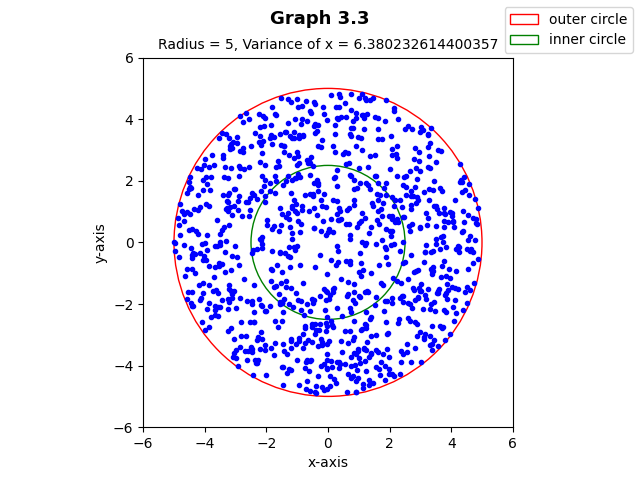
\includegraphics[scale=0.7]{Prob-Project/Q3/Q3(3).png}
\end{figure}
\end{document}